% ------------------------------------------------------------------------------
% TYPO3 CMS 8.5 - What's New - Chapter "In-Depth Changes" (Dutch Version)
%
% @author	Michael Schams <schams.net>
% @license	Creative Commons BY-NC-SA 3.0
% @link		http://typo3.org/download/release-notes/whats-new/
% @language	English
% ------------------------------------------------------------------------------
% LTXE-CHAPTER-UID:		5ebcecbe-66abfa57-cf38bc00-aa637965
% LTXE-CHAPTER-NAME:	In-Depth Changes
% ------------------------------------------------------------------------------

\section{Systeemwijzigingen}
\begin{frame}[fragile]
	\frametitle{Systeemwijzigingen}

	\begin{center}\huge{Hoofdstuk 3:}\end{center}
	\begin{center}\huge{\color{typo3darkgrey}\textbf{Systeemwijzigingen}}\end{center}

\end{frame}

% ------------------------------------------------------------------------------
% LTXE-SLIDE-START
% LTXE-SLIDE-UID:		11c6ff27-1c351ee4-ad53fe01-b984cb81
% LTXE-SLIDE-ORIGIN:	bde270e6-ffef8544-ea472ed5-89ba8c3d English
% LTXE-SLIDE-TITLE:		#78581: FormEngine Data Providers
% ------------------------------------------------------------------------------

\begin{frame}[fragile]
	\frametitle{Systeemwijzigingen}
	\framesubtitle{FormEngine Data Providers}

	\begin{itemize}
		\item De FormEngine data provider \texttt{TcaFlexFetch} is samengevoegd in \texttt{TcaFlexPrepare}
		\item Dit is alleen van invloed in het onwaarschijnlijke geval dat een eigen data-provider een afhankelijkheid heeft
			met \texttt{TcaFlexFetch}
	\end{itemize}

\end{frame}

% ------------------------------------------------------------------------------
% LTXE-SLIDE-START
% LTXE-SLIDE-UID:		39e83080-e9ea031d-41791964-42923212
% LTXE-SLIDE-ORIGIN:	f0fb603c-54e9f255-03140395-b6b18103 English
% LTXE-SLIDE-TITLE:		#78384: Frontend ignores TCA in ext_tables.php
% ------------------------------------------------------------------------------
\begin{frame}[fragile]
	\frametitle{Systeemwijzigingen}
	\framesubtitle{TCA in \texttt{ext\_tables.php}}

	\begin{itemize}
		\item Frontend aanroepen laden niet langer \texttt{ext\_tables.php}
		\item Deze wijziging is van invloed op extensies die TCA in  \texttt{ext\_tables.php} definiëren\newline
			\small(wat sowieso niet toegestaan is)\normalsize
		\item Install Tool heeft een test "TCA ext\_tables controle" om zulke extensies op te sporen
	\end{itemize}

	\begin{figure}
		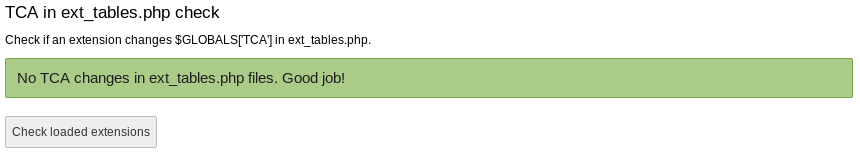
\includegraphics[width=0.95\linewidth]{InDepthChanges/78384-install-tool-tca-in-exttables-check.png}
	\end{figure}

\end{frame}
% ------------------------------------------------------------------------------
% LTXE-SLIDE-START
% LTXE-SLIDE-UID:		d62f24fc-10072c27-e92c96ae-6bc46a14
% LTXE-SLIDE-ORIGIN:	bdcd2449-b679717b-9f23eb32-018953b4 English
% LTXE-SLIDE-TITLE:		#78191: Remove support for transForeignTable/transOrigPointerTable in TCA
% ------------------------------------------------------------------------------
\begin{frame}[fragile]
	\frametitle{Systeemwijzigingen}
	\framesubtitle{TCA in \texttt{ext\_tables.php}}

	\begin{itemize}
		\item Database tabellen die vertaalde records bevatten waren te configureren in de TCA

			\begin{itemize}
				\item \texttt{\$TCA[<tabelnaam>]['ctrl']['transForeignTable']}\newline
					(wees meestal naar tabel: \texttt{pages\_language\_overlay})
				\item \texttt{\$TCA[<tabelnaam>]['ctrl']['transOrigPointerTable']}\newline
					(wees meestal naar tabel: \texttt{pages})
			\end{itemize}

		\item Deze configuratie is gewijzigd in direct tabelnamen om speciale afhandeling te voorkomen en als voorbereiding voor
			het samenvoegen van beide tabellen in de toekomst

	\end{itemize}

\end{frame}

% ------------------------------------------------------------------------------
% LTXE-SLIDE-START
% LTXE-SLIDE-UID:		3571c7b7-114dd3e2-a15bef73-d8ee9cd4
% LTXE-SLIDE-ORIGIN:	ede02440-cafd3417-eb416f09-8e024ef2 English
% LTXE-SLIDE-TITLE:		#78383: Tables removed from defaultCategorizedTables
% ------------------------------------------------------------------------------
\begin{frame}[fragile]
	\frametitle{Systeemwijzigingen}
	\framesubtitle{Tabellen verwijderd uit \texttt{defaultCategorizedTables}}

	\begin{itemize}
		\item De volgende tabellen zijn verwijderd uit \texttt{defaultCategorizedTables}:

			\begin{itemize}
				\item \texttt{pages}
				\item \texttt{tt\_content}
				\item \texttt{sys\_file\_metadata}
			\end{itemize}

		\item Voor deze tabllen wordt de core API\newline
			\texttt{ExtensionManagementUtility::makeCategorizable()}\newline
			aangeroepen om een algemene positie van het categorieveld te definiëren

	\end{itemize}

\end{frame}


% ------------------------------------------------------------------------------
% LTXE-SLIDE-START
% LTXE-SLIDE-UID:		56bf6d24-bff01e7b-0e30d986-b22c86a3
% LTXE-SLIDE-ORIGIN:	dd31e5d5-ca09ae5e-eb87d926-0ffe8f0a English
% LTXE-SLIDE-TITLE:		Low-level parameters changes (1)
% ------------------------------------------------------------------------------
\begin{frame}[fragile]
	\frametitle{Systeemwijzigingen}
	\framesubtitle{Parameterwijzigingen in Low-level (1)}

	% changes: #78417, #78439, #78520, #78552, #78577, #78623, #78627 and #78895

	\begin{itemize}
		\item Low-level commando's in de lijst hieronder gebruiken nu de Symfony Console
		\item Nieuwe commando's werken zoals de oude, maar ondersteunen bepaalde parameters

			\begin{itemize}
				\item \texttt{DeletedRecordsCommand}
				\item \texttt{CleanFlexFormsRecordsCommand}
				\item \texttt{OrphanRecordsCommand}
				\item \texttt{LostFilesCommand}
				\item \texttt{MissingFilesCommand}
				\item \texttt{MissingRelationsCommand}
				\item \texttt{DoubleFilesCommand}
				\item \texttt{RteImagesCommand}
			\end{itemize}

	\end{itemize}

\end{frame}



% ------------------------------------------------------------------------------
% LTXE-SLIDE-START
% LTXE-SLIDE-UID:		1ac92773-99aa4ddb-0131f01d-66beaf6a
% LTXE-SLIDE-ORIGIN:	3a9d25bb-d948368d-e2a92666-6170eaad English
% LTXE-SLIDE-TITLE:		Low-level parameters changes (2)
% ------------------------------------------------------------------------------
\begin{frame}[fragile]
	\frametitle{Systeemwijzigingen}
	\framesubtitle{Parameterwijzigingen in Low-level (2)}

	% changes: #78417, #78439, #78520, #78552, #78577, #78623, #78627 and #78895

	\begin{itemize}
		\item Gerelateerde PHP klassen zijn verwijderd\newline
			\smaller(e.g. \texttt{TYPO3\textbackslash
				CMS\textbackslash
				Lowlevel\textbackslash
				DeletedRecordsCommand})
			\normalsize

		\item Het commando via \texttt{cli\_dispatch} werkt niet meer\newline
			\smaller(bijv. \texttt{typo3/cli\_dispatch lowlevel cleaner deleted})\normalsize
		\item Aanroepen van de PHP klasse geeft nu een PHP-fout

		\item Commando's kunnen nu uitgevoerd worden via CLI als volgt:\newline
			\smaller\texttt{/typo3/sysext/core/bin/typo3 cleanup:<command>}\normalsize\newline
			bijvoorbeeld:\newline
			\smaller\texttt{/typo3/sysext/core/bin/typo3 cleanup:deletedrecords}\normalsize

	\end{itemize}

\end{frame}




% ------------------------------------------------------------------------------
% LTXE-SLIDE-START
% LTXE-SLIDE-UID:		54fa8078-94a5577b-b640736b-2b91059b
% LTXE-SLIDE-ORIGIN:	ec6817fd-c3364ffb-c74e9523-a18a3095 English
% LTXE-SLIDE-TITLE:		Re-factor FlexForm Data Structure Handling
% ------------------------------------------------------------------------------
\begin{frame}[fragile]
	\frametitle{Systeemwijzigingen}
	\framesubtitle{Herbouw afhandeling FlexForm Data Structure}

	% https://forge.typo3.org/issues/78581
	% https://forge.typo3.org/issues/78616
	% https://forge.typo3.org/issues/78852
	% https://forge.typo3.org/issues/69715

	\begin{itemize}
		\item Met de veroudering van \texttt{BackendUtility::getFlexFormDS()} wordt de hook
			\texttt{getFlexFormDSClass} niet langer aangeroepen

	\end{itemize}

\end{frame}





% ------------------------------------------------------------------------------
% LTXE-SLIDE-START
% LTXE-SLIDE-UID:		f19bd1cb-c1e95d77-7689b0c8-5749025d
% LTXE-SLIDE-ORIGIN:	b400c3b8-3e402480-cd7d6ff3-96cd93aa English
% LTXE-SLIDE-TITLE:		#76085: Add fluid debug information to admin panel
% ------------------------------------------------------------------------------
\begin{frame}[fragile]
	\frametitle{Systeemwijzigingen}
	\framesubtitle{Admin Panel}

	\begin{itemize}
		\item Admin Panel heeft een nieuwe optie om Fluid uitvoer te debuggen:\newline
			\textbf{Preview -> Show fluid debug output}
		\item Indien ingeschakeld worden de volgende details getoond:

			\begin{itemize}
				\item pad naar het sjabloonbestand van een partial
				\item naam van de section
			\end{itemize}

		\item Hiermee kunnen integrators eenvoudig de juiste sjabloon en section vinden

	\end{itemize}

\end{frame}






% ------------------------------------------------------------------------------
% LTXE-SLIDE-START
% LTXE-SLIDE-UID:		bfa77eba-d53bb364-7ff3a912-7d616634
% LTXE-SLIDE-ORIGIN:	60a2d39f-f04b8bf1-dc758912-607ed07e English
% LTXE-SLIDE-TITLE:		#52286: System Status Updates Report via email
% ------------------------------------------------------------------------------
\begin{frame}[fragile]
	\frametitle{Systeemwijzigingen}
	\framesubtitle{Systeemstatus updates (rapportages)}

	\begin{itemize}
		\item Resultaten van tests in "Systeemstatus Updates (rapportages)" kunnen doorgemaild worden
		\item Een keuzevakje is toegevoegd aan de taakconfiguratie om:

			\begin{itemize}
				\item een e-mail te sturen als er waarschuwingen of foutmeldingen zijn
				\item altijd een e-mail te maken
			\end{itemize}

		\item Standaard worden alleen waarschuwingen en fouten opgenomen

	\end{itemize}

\end{frame}







% ------------------------------------------------------------------------------
% LTXE-SLIDE-START
% LTXE-SLIDE-UID:		70734912-aba31c23-48ef958c-cdfc7ea6
% LTXE-SLIDE-ORIGIN:	e4e2ead3-c07beb21-e8100580-d0e7c756 English
% LTXE-SLIDE-TITLE:		#58637: Purge language packs in language module
% ------------------------------------------------------------------------------
\begin{frame}[fragile]
	\frametitle{Systeemwijzigingen}
	\framesubtitle{Taalpakketten}

	\begin{itemize}
		\item Uitschakelen van talen in de module "Talen" liet de taaldata achter
			in de map \texttt{typo3conf/l10n/<locale>/}
		\item Een knop "verwijderen" is toegevoegd die de taal uitschakelt en de data
		 	in de map verwijdert
	\end{itemize}

\end{frame}








% ------------------------------------------------------------------------------
% LTXE-SLIDE-START
% LTXE-SLIDE-UID:		4fcbe168-45481d20-2fad5c94-2e8a3f64
% LTXE-SLIDE-ORIGIN:	08961fb3-00cbc9f4-964f8d01-6e59e782 English
% LTXE-SLIDE-TITLE:		#67909: Hook added to localize() function
% ------------------------------------------------------------------------------
\begin{frame}[fragile]
	\frametitle{Systeemwijzigingen}
	\framesubtitle{Hook in DataHandler \texttt{localize()}}

	% decrease font size for code listing
	\lstset{basicstyle=\tiny\ttfamily}

	\begin{itemize}
		\item Een nieuwe hook is toegevoegd aan de functie \texttt{localize()}
		\item Hiermee kunnen externe vertaalservices of maatwerk tekensetomzettingen content transformeren
	\end{itemize}

	\begin{itemize}
		\item Hook:\newline
			\smaller
				\texttt{\$GLOBALS['TYPO3\_CONF\_VARS']['SC\_OPTIONS']\newline
				\tabto{0.4cm}['t3lib/class.t3lib\_tcemain.php']['processTranslateToClass']}
			\normalsize

		\item Voorbeeldgebruik:

			\begin{lstlisting}
				class YourHookClass
				{
				  public function processTranslateTo_copyAction(&$content, $lang, $dataHandler)
				  {
				    // Doe iets met content (translate, transliterate etc.)
				  }
				}
			\end{lstlisting}
	\end{itemize}

\end{frame}









% ------------------------------------------------------------------------------
% LTXE-SLIDE-START
% LTXE-SLIDE-UID:		67c9664e-e3ce6520-e8b7408e-e7733d61
% LTXE-SLIDE-ORIGIN:	8b1a9661-d6fab90f-9c856224-ee663aa2 English
% LTXE-SLIDE-TITLE:		#77757: Re-check if an UpdateWizard should run
% ------------------------------------------------------------------------------
\begin{frame}[fragile]
	\frametitle{Systeemwijzigingen}
	\framesubtitle{Update-assistent}

	\begin{columns}[T]
		\begin{column}{.5\textwidth}
			De Update-assistent in de Install Tool geeft een overzicht van taken die \textit{afgerond} zijn.
			\newline\newline
			Keuzevakjes en een knop "Recheck chosen wizards" zorgen ervoor dat updates opnieuw uitgevoerd kunnen worden.
			De assistent test zelf of de taak opnieuw uitgevoerd moet worden.
		\end{column}
		\begin{column}{.5\textwidth}
			\begin{figure}\vspace*{-0.5cm}
				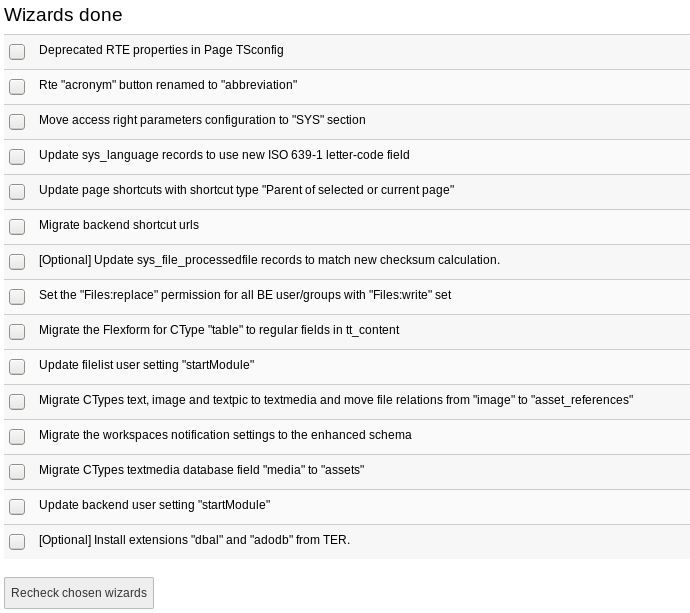
\includegraphics[width=0.8\linewidth]{InDepthChanges/77757-upgrade-wizard.png}
			\end{figure}
		\end{column}
	\end{columns}

\end{frame}









% ------------------------------------------------------------------------------
% LTXE-SLIDE-START
% LTXE-SLIDE-UID:		c5647fc5-ff651010-49912323-54dfe36f
% LTXE-SLIDE-ORIGIN:	94640f3d-0f632507-a2166719-5adc755e English
% LTXE-SLIDE-TITLE:		#78523: Suggest wizard provides option to define ordering of results
% ------------------------------------------------------------------------------
\begin{frame}[fragile]
	\frametitle{Systeemwijzigingen}
	\framesubtitle{Suggestie-assistent}

	% decrease font size for code listing
	\lstset{basicstyle=\tiny\ttfamily}

	\begin{itemize}
		\item De FormEngine ("TCEforms") laat nu de volgorde van de suggesties instellen
		\item De nieuwe optie is een standaard SQL order-by definitie:\newline
			\small\texttt{'orderBy' => 'field ASC/DESC'}\normalsize
		\item Voorbeeld TCA-configuratie:

			\begin{lstlisting}
				'config' => [
				  ...
				  'wizards' => [
				    'suggest' => [
				      'type' => 'suggest',
				      'default' => [
				        'searchWholePhrase' => true,
				        'addWhere' => ' AND tx_news_domain_model_news.uid != ###THIS_UID###',
				        'orderBy => 'datetime DESC',
				      ]
				    ],
				  ],
				]
			\end{lstlisting}

	\end{itemize}

\end{frame}











% ------------------------------------------------------------------------------
% LTXE-SLIDE-START
% LTXE-SLIDE-UID:		13c3abe1-610d5d72-56d110f3-1a3fa949
% LTXE-SLIDE-ORIGIN:	0907e5d3-a12751cb-23f49488-7a05a208 English
% LTXE-SLIDE-TITLE:		Miscellaneous
% ------------------------------------------------------------------------------
\begin{frame}[fragile]
	\frametitle{Systeemwijzigingen}
	\framesubtitle{Divers}

	% #78103: Add missing information status for addSystemMessage
	% #78575: Get enumeration constants
	% #75232: Spread TypeConverter priorities

	\begin{itemize}
		\item Alle systeeminformatie toegevoegd door \texttt{addSystemInformation()} heeft nu
			\texttt{InformationStatus::STATUS\_NOTICE} als standaard waarde
		\item De opsommingsconstanten kunnen nu eenvoudig opgehaald worden:

			\begin{itemize}
				\item \texttt{EnumerationClass::getName(\$value);}
				\item \texttt{EnumerationClass::getHumanReadableName(\$value);}
			\end{itemize}

		\item Prioriteiten van de TypeConverters uit de core zijn gewijzigd van \newline
			\texttt{1}, \texttt{2}, \texttt{3},... in \texttt{10}, \texttt{20}, \texttt{30},...
			Let bij het registreren van maatwerk TypeConverters op de juiste prioriteiten.

		\item \href{https://en.wikipedia.org/wiki/ISO_8601}{ISO-8601} wordt nu gebruikt om date en datetime
			waardes door te geven tussen server en de client. Eventueel moeten maatwerk FormEngine rendertypes
			bijgewerkt worden (\texttt{eval=date/datetime}).

	\end{itemize}

\end{frame}












% ------------------------------------------------------------------------------
